\documentclass[12pt,a4paper,twoside,openright]{report}

\usepackage{cs}
\usepackage{amsthm}
\theoremstyle{definition}
\newtheorem{defi}{Definiție}
\theoremstyle{remark}
\newtheorem{ex}{Exemplu}

\usepackage[english,romanian]{babel}

\graphicspath{{figures/}}
\ifpdf
  \DeclareGraphicsExtensions{.pdf,.jpeg,.png}
\else
  \DeclareGraphicsExtensions{.eps}
\fi

\mastersthesis
\singlespace

\renewcommand{\thesisauthor}{Adrian Bona}
\renewcommand{\thesismonth}{Iunie}
\renewcommand{\thesisyear}{2015}
\renewcommand{\thesistitle}{Metodă pentru silabisirea cuvintelor folosind tipare secvențiale frecvente}

\renewcommand{\thesissupervisorname}{Prof. dr. ing. Rodica Potolea}
\begin{document}

\begin{titlepage}

\thispagestyle{firststylewithoutfooter}

\begin{center}
{\scshape \facultynameromanian} \\
{\scshape \departmentnameromanian} \\


\vspace{6cm}

\thesistitlesize {\textbf{\thesistitle}\\}

\vspace {1cm}

\Large \textbf{\thesistyperomanian}\\

\vspace{2cm}

\thesisauthortypesize \thesisauthortyperomanian \\ \textbf{\thesisauthor} \\

\vspace{1cm}

\thesissupervisorsize \thesissupervisorromanian \\ \textbf{\thesissupervisorname}\\



\vspace{\stretch{1}}
{\thesismonth} {\thesisyear} \\
\end{center}
\end{titlepage}

\begin{titlepage}
\phantom{1}
\end{titlepage}

\begin{titlepage}

\begin{center}

\thispagestyle{firststylewithfooter}

{\scshape \facultynameromanian} \\
{\scshape \departmentnameromanian} \\

\vspace{1cm}

\newcolumntype{R}{>{\raggedleft\arraybackslash}X}%
\begin{tabularx}{\textwidth}{lR}
{\scshape \facultydeanromanian} & {\scshape \deptmanagerromanian} \\
\facultydeanname & \deptmanagername\\
\end{tabularx}

\vspace {2cm}

\thesistitlesize {\textbf{\thesistitle}\\}
\vspace {1cm}

\thesistypesize \textbf{\thesistyperomanian}\\

\vspace{1cm}

\end{center}

\begin{flushleft}
\begin{enumerate}
  \item \thesisauthortyperomanian: \thesisauthor
  \item \thesissupervisorromanian: \thesissupervisorname
  \item \thesiscontentsromanian: Pagina de prezentare, aprecierile coordonatorului, titlul capitolului 1, titlul capitolului 2, \dots, titlul capitolului n, bibliografie, anexe, CD.
  \item \thesisworkingplaceromanian: UTCN, Cluj-Napoca
  \item \thesisadvisorsromanian: dr. ing Camelia Lemnaru
  \item \thesisbegindateromanian: \dotfill
  \item \thesisenddateromanian: \dotfill
\end{enumerate}
\end{flushleft}

\vspace{0.5cm}

\begin{center}

\newcolumntype{R}{>{\raggedleft\arraybackslash}X}%
\begin{tabularx}{\textwidth}{lR}
{\thesissignatureromanian} {\thesissupervisorromanian} & {\thesissignatureromanian} {\thesisauthortyperomanian} \\
\thesissupervisorname & \thesisauthor \\
\end{tabularx}

\vspace{\stretch{1}}
{\thesismonth} {\thesisyear} \\

\end{center}

\end{titlepage}

\begin{titlepage}
\phantom{1}
\end{titlepage}

\begin{titlepage}

\begin{center}
\thispagestyle{firststylewithfooter}
{\scshape \facultynameromanian} \\
{\scshape \departmentnameromanian} \\
\end{center}

\vspace{3cm}

\begin{center}
\autheticitydeclarationsize \textbf{\autheticitydeclarationromanian}
\end{center}

\vspace{1cm}

Subsemnatul \textit{\thesisauthor}, legitimat cu \textit{CI/BI} seria \textit{XX} numărul \textit{NNNNNN}, CNP \textit{LLLLLLLLLLLL}, autorul lucrării \textit{\thesistitle} elaborată în vederea susținerii examenului de finalizare a studiilor de masterat la Facultatea de Automatică și Calculatoare, Departamentul Calculatoare, Specializarea \textit{SSSSSSSS} din cadrul Universității Tehnice din Cluj-Napoca, sesiunea \textit{\thesismonth} a anului univeristar \textit{20XX/20XX}, declar pe proprie răspundere, că această lucrare este rezultatul propriei mele activități intelectuale, pe baza cercetărilor mele și pe baza informatiilor obținute din surse care au fost citate în textul lucrării și în bibliografie.

Declar că această lucrare nu conține porțiuni plagiate, iar sursele bibliografice au fost folosite cu respectarea legislației române și a convențiilor internaționale privind drepturile de autor.

Declar, de asemenea, că această lucrare  nu a mai fost prezentată în fața unei alte comisii de examen de licență sau disertație.

În cazul constatării ulterioare a unor declarații false, voi suporta sancțiunile administrative, respectiv, \textit{anularea examenului de disertație}.


\vspace{2cm}

\begin{center}

\newcolumntype{R}{>{\raggedleft\arraybackslash}X}%
\begin{tabularx}{\textwidth}{lR}
Cluj-Napoca & {\thesissignatureromanian}\\
data  & {\thesisauthortyperomanian} \\ 
\end{tabularx}

\end{center}

\end{titlepage}

\begin{titlepage}
\phantom{1}
\end{titlepage}

\begin{abstract}
\end{abstract}

\begin{titlepage}
\phantom{1}
\end{titlepage}

\pagenumbering{roman}
\setcounter{page}{1}

\tableofcontents
\newpage

\listoftables
\listoffigures

\newpage

\pagenumbering{arabic}
\setcounter{page}{1}

\setlength{\headheight}{15pt}

\pagestyle{fancy}
\renewcommand{\chaptermark}[1]{ \markboth{\thechapter. #1}{} }
\renewcommand{\sectionmark}[1]{ \markright{\thesection. #1}{} }

\renewcommand{\headrulewidth}{1pt}
\renewcommand{\footrulewidth}{1pt}


\fancyhf{}
\fancyhead[LE]{\textit{ \nouppercase{\leftmark}} }
\fancyhead[RO]{\textit{ \nouppercase{\rightmark}} }
\fancyfoot[RE]{{\thesismonth} {\thesisyear}}
\fancyfoot[LE,RO]{\thepage}

\fancypagestyle{plain}{ %
  \fancyhf{}
  \renewcommand{\headrulewidth}{0pt}
  \renewcommand{\footrulewidth}{1pt}
  \fancyfoot[LE,RO]{\thepage}
}



\chapter{Introducere}
\label{cap:Introducere}
În cadrul acestui proiect se încearcă identificarea unei metode care rezolvă problema silabificării. 

O astfel de metodă este de interes într-o serie de domenii conexe lingvisticii, spre exemplu în cadrul editoarelor de text sau pentru sinteza artificială a limbajului (audio).

Soluția propusă se folosește de metode de învățare supervizată bazându-se tipare secventiale. 

Ce se scrie aici:
\begin{itemize}
    \item Contextul
    \item Conturarea/Descrierea domeniului exact al temei
    \item Se răspunde la întrebările: \textbf{ce} (s-a făcut)?, \textbf{de ce} (s-a făcut, adică motivația; ce se rezolvă, la ce este util, etc.)?, \textbf{cum} (s-a făcut, adică particularitățile abordării, prezentate sumar).
    \item Introducerea se termină cu o descriere a conținutului lucrării, de genul: Cap X descrie ..., Cap Y prezintă ...
    \item Introducerea reprezintă o sinteză a lucrării, din care cititorul trebuie să-și poată da bine seama dacă lucrarea prezintă sau nu interes pentru el. 
    \item Se poate organiza pe subsecțiuni, dacă se dorește, după exemplul de mai jos, dar nu e obligatoriu asta, având în vedere dimensiunea mică
    \item reprezintă cca 5\% din lucrare (nu mai mult de 2-4 pagini)
\end{itemize}

\section{Context}

Despre contextul în care este abordată și se aplică tema lucrării.

% \section{Motivation}
\section{Motivație}
De ce este utilă abordarea temei? Ce probleme rezolvă și ce rezultate poate aduce?

% \section{Report's Structure}
\section{Structura lucrării}
Capitolul~\ref{cap:obiective-specificatii} prezintă obiectivele \dots. Capitolul~\ref{cap:studiu-bibliografic} descrie \dots. În capitolul~\ref{cap:fund-teoretice} sunt prezentate \dots.

\chapter{Obiective}
\label{cap:obiective-specificatii}
\section{Obiective}
Contribuția principală asteptată de la acest proiect ține de dezvoltarea unei metode prin care se pot obține silabisiri ale cuvintelor scrise, cu precizie ridicată. 

Pe lângă acest obiectiv general trebuie avute în vedere și următoarele cerințe: 

\begin{itemize}
\item \textit{Genericitate la nivel de limba}. Se urmărește o identificarea unei soluții generale, care să funcționeze cel puțin la nivelul unei familii de limbi.
\item \textit{Scalabilitate la nivelul timpului de execuție}. Este necesar ca despărțirile în silabe să se realizeze cât mai rapid posibil, mai ales în contextul sintezei de voce. 
\item \textit{Înglobarea excepțiilor lingvistice în cadrul soluției}. Acest obiectiv, deși antitetic cu primul, trebuie cel puțin avut în vedere.
\item \textit{Tratarea silabificărilor dependente de context}. Cel puțin în cadrul limbii române, despărțirea în silabe poate fi ambiguă, depinzând de contextul în care este realizată.
\item \textit{Identificarea unui set de metrici pentru validarea rezultatelor.}

\end{itemize}

\chapter{Studiu bibliografic}
\label{cap:studiu-bibliografic}

În cadrul acestui capitol, problema silabisirii va fi încadrată într-o categorie mai generală de probleme și vor fi referite o serie de articole în care sunt descris soluții propuse urmând ca în ultima parte să fie referite o serie de articole din din domeniul extragerii de cunostințe sub formă de tipare secvențiale frecvente.

\section{Silabisirea ca problemă de învațare automată}

Sibabisirea ca problemă poate fi privită din două perspective: în primul rând este necesară o clarificare a conceptului de silabisire (avem silabisire ortografică și silabisire fonetică) iar al doilea motiv ține de problema în sine a prezicerii punctelor de despărțire în silabe ale unui cuvânt. 

Performanța oricărei soluții depinde în mare măsură de definirea clară a problemei. Odată eliminată ambiguitatea cerințelor se pot construi soluții. Fiind o problema în care se cer o serie de predictii, este necesară construirea unui model general, care sa fie folosit pentru a realiza aceste predicitii. Ajunși aici, putem considera problema ca fiind una de învățare automată, iar învățarea automată poate fi realizată, în general, în două feluri: învățare automată supervizată sau învățare automată nesupervizată. 

Învătarea automată supervizată presupune că modelul folosit pentru predicții este construit din exemple de predicție. Învătarea automată nesupervizată construieste modele de predicție fără a avea exemple. 

\section{Soluții propuse pentru problema silabisirii}

În contextul problemei de silabisire, în cadrul ~\cite{bib:marchand2009automatic} se realizeaza o sinteza a soluțiilor curente pentru limba engleză și se definesc doua clase de soluții: soluții bazate pe învătare automată supervizată și soluții bazate pe reguli. Soluțiile bazate pe reguli prezintă un mare dezavantaj, deoarece regulile sunt dependente de limbă, si este necesară o bună cunoastere a limbii respective din partea celui care implementează o astfel de soluție.

Pentru soluții independente de limba, în ~\cite{bib:liang1983word} este prezentată o metodă pentru silabisirea ortografică care stă la baza sistemului \LaTeX și care se folosește de o serie de tipare si anti-tipare pentru a realiza predicții de despărțiri în silabe. O altă metodă îndependentă de limbă este prezentată în cadrul ~\cite{bib:kiraz1998multilingual}, unde se utilizeaza automate finite. 

Din perspectiva recunoașterii vorbirii, în cadrul ~\cite{bib:hunt1980experiments} este prezentată posibilitatea identificării silabelor din secvențe de sunete, iar în ~\cite{bib:damper1997pronunciation} este propusă o metodă de sinteză a vorbirii bazată pe analogie, care poate fi folosită ca model pentru o soluție de silabisire la nivel de limbaj scris. 

\section{Soluții de silabisire pentru limba română}

Pentru limba română, au fost propuse o serie de soluții pentru această problemă, în cadrul ~\cite{bib:dinu2004despartirea} fiind descrisă construcția unei baze de date a silabelor limbii române, iar în ~\cite{bib:barbu2008romanian} este descrisă un dicționar pentru despărțiri în silabe în care se are în vedere și ambiguitatea anumitor despărțiri în functie morfologia cuvintelor. Ulterior, s-au realizat și o serie de experimente folosind tehnici de învățare automată pentru a rezolva problema silabisirii, aceastea fiind descrise în ~\cite{bib:dinu2013romanian}.


\section{Tipare secvențiale}

Din perspectiva secvențialitătii silabelor se pot urmării tehnici generale de extragere de tipare frecvente secvențiale descrise în \cite{bib:agrawal1995mining} sau soluții mai recente cum ar fi algoritmul BIDE, descris în \cite{bib:wang2004bide} sau gapBIDE \cite{bib:gapbide} o variantă a aceluiași algoritm care permite identificarea de tipare cu goluri. 

Pe scurt, aceste tehnici încearcă să identifice posibile tipare frecvente dintr-o colecție de secvente, pornind de la subsecvențe frecvente de dimensiune redusă si extinzându-le pe acestea în mai multe rânduri. Aplicațiile pentru aceste tipare pot fi diverse, dar dintre acestea pot fi mentionațe câteva: detecția tiparelor de intrusiune, detecția de secvențe de instrucțiuni de programe care conțin defecte sau detecția tiparelor de comportament ale utilizatorilor în cadrul aplicațiilor web sau din cadrul telefoanelor inteligente.

\section{Algoritmi de cautare în siruri de caractere}

Acest subiect este de interes într-o în vederea identificării prezentei unor tipare secvențiale frecvente în cadrul cuvintelor, care sunt reprezentate prin siruri de caractere. Soluția naivă la această problemă presupune identificarea tuturor sub-șirurilor de caractere si verificarea ca unul dintre sub-șiruri să fie cel cautat. În \cite{bib:knuth1977fast} este prezentat un algoritm clasic care rezolva această problema, iar în  \cite{bib:baeza1992new} și \cite{bib:baeza1996faster} sunt prezentate alte două soluții de căutare aproximativă.


\chapter{Fundamente teoretice}
\label{cap:fund-teoretice}

În cadrul acestui capitol vor fi prezentate elementele care stau la baza metodei descrise în cadrul acestui proiect. În primele doua secțiuni vor fi definite despărțirea în silabe și tiparele secvențiale, urmând ca în a treia secțiune să fie definit conceptul de tipar secvențial frecvent la nivelul cuvintelor.

\section{Despărțirea în silabe (silabisirea)}

Prin silabisire se înțelege a procesul de a despărți în silabe un cuvânt. Înainte de a oferi câteva exemple, este necesară o clarificare a conceptului de silabă. 

\begin{defi}
\textbf{Silaba} se definește ca fiind un segment din lanțul vorbirii compus din unul sau mai multe foneme (sunete elementare) pronunțate neîntrerupt într-un singur efort respirator. Orice silabă are ca element principal inevitabil o vocală sau, în unele limbi, o consoană sonantă). Elementul principal poate fi însoțit de consoane, semivocale sau grupuri consonantice și semivocalice dispuse înainte, după, sau de ambele părți ale acestuia. \footnote{http://ro.wikipedia.org/wiki/Silabă}
\end{defi} 

Deasemenea, trebuie menționat că silabisirea nu poate fi definită pe baza unui set rigid de reguli, chiar dacă în majoritatea cazurilor există un asemenea set de reguli. Această ambiguitate la nivelul definirii procesului vine din două cauze: 
\begin{enumerate}
\item limbile nu sunt construite artificial, iar ambiguitatea este un atribut intrinsec al lor. 
\item silabisirea este realizată după seturi diferite de reguli, în functie de scopul pentru care este realizată (fonetic sau ortografic).  
\end{enumerate}

Silabisirea fonetică ilustrează cel mai bine definiția de mai sus, dar când vine vorba de silabisirea ortografică trebuie mentionat ca principala utilitate a acestui tip de despărțire în silabe este acela estetic.

\begin{ex}
Din punct de vedere fonetic, despărțirea în silabe a cuvântul \textit{inegal} este \textbf{i-ne-gal}, dar din punct de vedere ortografic, utilizând reguli morfologice rezultă despărțirea \textbf{in-e-gal}. 
\end{ex}

\section{Tipare secventiale frecvente}

Tiparele secventiale frecvente sunt acele tipare care se regasesc în cadrul unei colecții de secvențe ordonate de numar minim de ori. Acest numar va fi referit ulterior și ca \textit{suport minim}. 

In cele ce urmeaza, se va realiza o introducere formală pentru tiparele secvențiale frecvente, urmând ca după această scurtă întroducere să fie ilustrat modul în care o colecție de cuvinte despărțite în silabe poate fi asociată cu o colecție de secvențe.

\begin{defi}
Fie $I = \{i_1, i_2, ...,i_n\}$ alfabetul (un set distinct de itemi) colecției de secvențe. O \textbf{secvență $S$} este definită ca fiind o listă ordonată de elemented din alfabetul $I$, $<i_{k_1},i_{k_2}, ...,i_{k_m}>$, unde $\forall k_j, 0 \leq j \leq m, k_j \epsilon I$. 
De exemplu, având alfabetul $I=\{a,b,c,d\}$, o posibilă secvență este $<b,b,a>$.
\end{defi}

\begin{defi} 
Printr-o \textbf{colecție de secvențe $S_{db}$} se înțelege un set de tuple de forma $(S_{id}, S)$, unde $S_{id}$ este un identificator unic iar $S$ este o secvență. 
\end{defi}

\begin{ex}
Un exemplu de astfel colecție de secvențe este prezentat în cadrul tabelului \ref{table:sdb}
\end{ex}

\begin{table}[h]
\centering    
\begin{tabular}{|c|c|}    
\hline      
$S_{id}$ & $S$ \\
\hline                    
1 & $<a,b,c,b,a>$ \\
2 & $<a,a,a,b,c>$ \\
3 & $<b,b,b,b,a>$ \\
4 & $<c,b,b,a>$ \\
\hline                              
\end{tabular}
\caption{Exemplu de colecție de secvențe}
\label{table:sdb}               
\end{table}

Despre o secvență $S_1=<t_1, t_2, ...,t_n>$ se poate spune ca este conținută de o secvență $S_2=<l_1, l_2, ...,l_m>$ dacă $n \leq m$ și $ \exists i,j$ astfel încât $t_1 = l_i, t_n = l_j$ și $\forall k, i \leq k \leq j \implies t_{k-i} = l_k$. Pentru această incluziune a secvențelor se va utiliza ulterior notația $S_1 \subseteq S_2$.      
\begin{defi}

Fie $S_{db}$ o colecție de secvențe, iar $T$ multimea tuplelor $(S_{id}, S)$ din $S_{db}$, pentru care $S' \subseteq S$. \textbf{Suportul} secvenței $S'$ în cadrul acestei colecții de secvențe este $\vert T \vert$.  Informal, suportul unei secvențe într-o colecție de secvențe este egal cu numarul de secvențe din acea colecție, care conțin secvența respectivă. Pentru suportul secvenței $S$ în cadrul $S_{db}$ se va utiliza notația $sup_{S_{db}}(S)$.
\end{defi}

Pornind de la definiția unei secvențe și a suportului unui secvențe se poate introduce conceptul de \textbf{tipar secvențial frecvent}. Un tipar secvențial frecvent nu este altceva decât o secvență care în cadrul unei colecții de secvențe $S_{db}$ are un suport mai mare sau egal cu un prag minim. Acest prag minin se mai numește și \textbf{suport minim}.

Identificare tiparelor descrise anterior prezintă un interes deosebit, cu aplicabilitate într-o multitudine de domenii, iar după cum va fi ilustrat în capitolele urmatoare, tiparele extrase din cuvinte deja despărțite în silabe pot fi utilizate pentru a construi strategii de predicție a silabisirii cuvintelor. 

\begin{ex}
Într-un astfel de scenariu în care se dorește identificarea tiparelor frecvente din cuvinte despărțite în silabe, alfabetul colecției de secvențe este reprezentat de mulțimea tuturor posibilelor silabelor, iar fiecare cuvânt reprezintă o secvență. În cadrul tabelului \ref{table:sdb_words} este prezentată o astfel de colecție de secvențe.
\end{ex}

\begin{table}[h]
\centering    
\begin{tabular}{|c|c|}    
\hline      
$S_{id}$ & $S$ \\
\hline
1 & \textit{<li, be, lu, lă>} \\
2 & \textit{<e, li, be, ra, tor>} \\
3 & \textit{<a, ma, tor>}\\
4 & \textit{<ar, ti, col>} \\
5 & \textit{<pro, gra, ma, tor>} \\
6 & \textit{<a, ni, ver, sa, re>} \\
7 & \textit{<vi, sa, re>} \\
8 & \textit{<gra, ma, ti, că>} \\
9 & \textit{<e, va, da, re>} \\
10 & \textit{<ma, re, e>} \\
11 & \textit{<pro, gra, ma, re>} \\
12 & \textit{<gân, di, tor>} \\
13 & \textit{<e, li, tă>} \\
14 & \textit{<sa, re>} \\
15 & \textit{<e, li, cop, ter>} \\
\hline                              
\end{tabular}
\caption{Exemplu de colecție de secvențe construite pe baza unui set de cuvinte despărțite în silabe}
\label{table:sdb_words}               
\end{table}

Pentru colecția de secvențe frecvente din cadrul tabelului \ref{table:sdb_words}, în cadrul tabelului \ref{table:sdb_patterns} sunt ilustrate tiparele frecvente în funcție de diferite valori ale suportului minim. Se va nota cu $(S,sup)$ un tipar frecvent, unde $S$ este tiparul propriu-zis iar $sup$ reprezintă valoarea suportului aceste secvente.

Tiparele identificate dintr-un set mare de cuvinte deja silabisite, pe lângă valoarea lor în contextul analizelor de fonetica și morfologie a limbi, pot fi folosite pentru a automatiza procesul de silabisire, asa cum va fi ilustrat în cadrul capitolului următor.

\begin{table}[h!]
\centering    
\begin{tabular}{|c|l|}    
\hline      
Suport minim & Tipar frecvent\\
\hline
2& $(<a>, 2)$  \\
 & $(<li, be>, 2)$  \\
 & $(<pro, gra, ma>, 2)$  \\
 & $(<ma, re>, 2)$  \\
 & $(<ma, tor>, 2)$  \\
 & $(<ti>, 2)$  \\
 & $(<e, li>, 3)$  \\
 & $(<gra, ma>, 3)$  \\
 & $(<sa, re>, 3)$  \\
 & $(<tor>,4)$  \\
 & $(<li>, 4)$  \\
 & $(<e>, 5)$  \\
 & $(<ma>,5)$  \\
 & $(<re>, 6)$  \\
\hline
3& $(<e, li>, 3)$  \\
 & $(<gra, ma>, 3)$  \\
 & $(<sa, re>, 3)$  \\
 & $(<tor>,4)$  \\
 & $(<li>, 4)$  \\
 & $(<e>, 5)$  \\
 & $(<ma>,5)$  \\
 & $(<re>, 6)$  \\
\hline
4& $(<tor>,4)$  \\
 & $(<li>, 4)$  \\
 & $(<e>, 5)$  \\
 & $(<ma>,5)$  \\
 & $(<re>, 6)$  \\
\hline
5& $(<e>, 5)$  \\
 & $(<ma>,5)$  \\
 & $(<re>, 6)$  \\
\hline
 & $(<re>, 6)$  \\
\hline                              
\end{tabular}
\caption{Exemplu de colecție de secvențe construite pe baza unui set de cuvinte despărțite în silabe}
\label{table:sdb_patterns}               
\end{table}

În cadrul sectiunii următoare se va face o scurtă prezentare a unuia dintre algoritmii performanți, cu ajutorul caruia se pot identifica tipare frecvente. 

\section{Algoritmul BIDE}
Algoritmul BIDE, prezentat în detaliu în \cite{bib:wang2004bide}, este o soluție capabilă să extragă tipare secventiale frecvente inchise.

\begin{defi}
Prin \textbf{tipar secvential închis} se întelege un tipar dintr-un set de tipare pentru care nu exista alt tipar care să-l conțină și să aiba același suport. Formal, $S$ este închis dacă $\forall S' \epsilon S_{db}, \nexists (S \subseteq S' \wedge sup_{S_{db}}(S)=sup_{S_{db}}(S'))$.
\end{defi}  

TODO... 
\chapter{De la tipare secventiale frecvente la silabisire}
\label{cap:contributii}

În cadrul acestui capitol se prezenta în detaliu metoda propusă, prin care, pornind de tipare secvențiale frecvente, se pot identifica despărțiri în silabe ale cuvintelor.  

\section{Prezentare de ansamblu a soluției}

\begin{figure}[h]
    \centering
    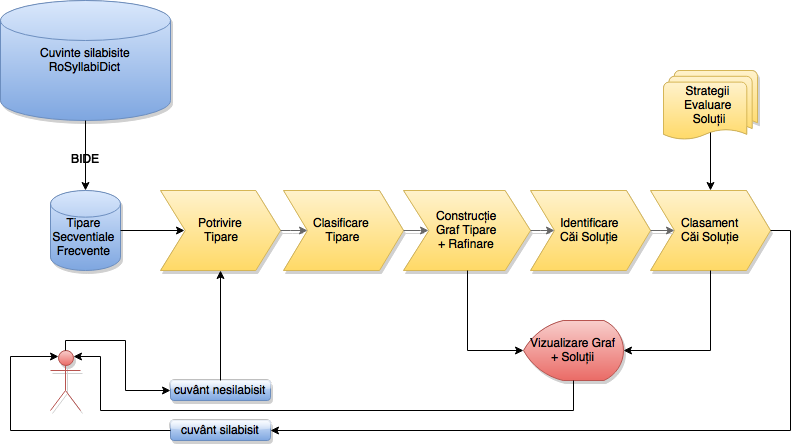
\includegraphics[width=\textwidth]{figures/rosil-flow.png}
    \caption{Diagrama conceptuală a soluției propuse}
    \label{fig:rosil-flow}
\end{figure}

Principalele etape ale metodei sunt următoarele:
\begin{enumerate}
\item Identificarea tiparelor frecvente dintr-un set de cuvinte despărțite în silabe și indexarea acestora.
\item Identificarea tiparelor care prezintă un grad ridicat de potrivire în cadrul cuvântului care se dorește a fi despărțit în silabe
\item Clasificarea acestor tipare în funcție poziția în cuvânt pe care au \textit{potrivit-o} (început, sfârșit, interior).
\item Construirea unui graf cu aceste tipare pe baza potrivirii dintre aceste tipare
\item Eliminarea nodurilor izolate din acest graf
\item Pe baza unor strategii de predicție, se va alege o cale sau mai multe în acest graf, reprezentând soluția propusă sau soluțiile soluțiile propuse pentru despărțirea în silabe.
\end{enumerate}

\section{Identificarea tiparelor frecvente}

Pentru a construi setul de tipare frecvente a fost folosită colecția de cuvinte despărțite în silabe în limba română RoSyllabiDict, \cite{bib:BARBU08.495}. Acest set de date conține 525486 de cuvinte despărțite în silabe. 

În vederea analizei setului de date, în cadrul tabelului \ref{table:sdb_counts} se poate observa variația numărului de tipare secvențiale frecvente închise în funcție de valoarea suportului minim.   

\begin{table}[h!]
\centering
\begin{tabular}{|c|c|c|c|c|c|c|c|c|}
\hline
Sup.& Total & Lung. 1 & Lung. 2 & Lung. 3 & Lung. 4 & Lung. 5 & Lung. 6 & Lung. 7\\ 
\hline
\hline
1000 & 648 & 252 & 385 & 11 & 0 & 0 & 0 & 0\\ 
\hline
800 & 890 & 293 & 576 & 21 & 0 & 0 & 0 & 0\\ 
\hline
600 & 1339 & 380 & 903 & 56 & 0 & 0 & 0 & 0\\ 
\hline
400 & 2211 & 523 & 1544 & 143 & 1 & 0 & 0 & 0\\ 
\hline
200 & 4812 & 832 & 3384 & 576 & 20 & 0 & 0 & 0\\ 
\hline
100 & 10461 & 1234 & 6754 & 2309 & 162 & 2 & 0 & 0\\ 
\hline
50 & 22852 & 1824 & 12671 & 7453 & 853 & 47 & 4 & 0\\ 
\hline
20 & 62549 & 2597 & 25731 & 28056 & 5384 & 674 & 90 & 17\\ 
\hline
10 & 129106 & 3271 & 41126 & 63388 & 17812 & 2940 & 454 & 97\\ 
\hline
5 & 256065 & 4146 & 63443 & 123429 & 52271 & 10553 & 1840 & 327\\ 
\hline
2 & 633195 & 5469 & 104254 & 248227 & 186623 & 66915 & 16920 & 3882\\ 
\hline\end{tabular}
\label{table:sdb_counts}
\caption{Numărul de tipare frecvente închise pentru setul de date RoSyllabiDict} 
\end{table}

Tiparele descrise in tabela precedentă au fost identificate folosind algoritmul BIDE, prin execuții succesive în care valoarea suportului minim a fost variată.

Alegerea unui suport minim cât mai mic asigură prezența a cât mai multor tipare în colecția de tipare folosite ulterior de metodă. Aceasta va creste precizia metodei, dar pe de altă parte va avea o influentă negativă asupra timpului de execuție. 

Cu cât numărul de tipare este mai mare, cautarea de potriviri devine mai lentă, iar pentru a creste performanța, acestea pot fi indexate. În tabelul \ref{table:sdb_patterns} sunt prezentate o serie de tipare frecvente. Pentru a le indexa metoda se folosește de o tabela de disperie în care valorile cheilor vor fi reprezentate de silabele concatenate continute de tipare. Un astfel de exemplu se regăseste în cadrul tabelului \ref{table:sdb_index}. 

\begin{table}[h!]
\centering    
\begin{tabular}{|l|l|}    
\hline      
Cheie & Valoare\\
\hline
$a$ 		& $(<a>, 2)$  \\
$libe$ 		& $(<li, be>, 2)$  \\
$programa$ 	& $(<pro, gra, ma>, 2)$  \\
$mare$ 		& $(<ma, re>, 2)$  \\
$mator$ 	& $(<ma, tor>, 2)$  \\
$ti$ 		& $(<ti>, 2)$  \\
$eli$ 		& $(<e, li>, 3)$  \\
$grama$ 	& $(<gra, ma>, 3)$  \\
$sare$ 		& $(<sa, re>, 3)$  \\
$tor$ 		& $(<tor>, 4)$  \\
$li$ 		& $(<li>, 4)$  \\
$e$ 		& $(<e>, 5)$  \\
$ma$ 		& $(<ma>, 5)$  \\
$re$ 		& $(<re>, 6)$  \\
\hline
\end{tabular}
\caption{Exemplu de indexare pentru tipare secvențiale frecvente}
\label{table:sdb_index}               
\end{table}  

Odată având colecția de tipare frecvente indexată, procesul de silabizarea poate fi initial. 
 
\section{Potrivirea tiparelor in vederea silabisirii}

Fie $w$ un cuvânt compus dintr-o secvență de litere, iar $Z_w$ mulțimea tuturor subsecventelor continue ale acestui cuvânt, precum si îndexii de inceput și sfârșit ai acestora.

\begin{ex}
Pentru cuvântul $amator$, tuplele din multimea sunt $Z_{amator}$ sunt ilustrate în cadrul tabelului \ref{table:sdb_substrings}. 
\end{ex}


\begin{table}[h!]
\centering    
\begin{tabular}{|l|l|}    
\hline      
Secventă & Indexi\\
\hline
$a$ 		& $\left[0,1\right), \left[2,3\right)$  \\
$m$ 		& $\left[1,2\right)$  \\
... 		& ...  \\
$amator$ 	& $\left[0,6\right)$  \\

\hline
\end{tabular}
\caption{Mulțimea $Z_{amator}$}
\label{table:sdb_substrings}               
\end{table}  

\begin{defi} Prin \textbf{potrivirea tiparelor} pentru cuvântul $w$, având multimea $Z_w$ asociată, se dorește identificarea tuturor tiparelor frecvente care sunt indexate cu chei care aparțin multimii $Z_w$. Notăm rezultatul acestei operații cu $M_w$. Considerând același cuvânt $amator$, $M_{amator}$ este ilustrată în tabelul \ref{table:sdb_pattern_match}
\end{defi}

\begin{table}[h!]
\centering    
\begin{tabular}{|l|l|}    
\hline      
Tipar frecvent & Indexi potrivire\\
\hline
$(<a>, 2)$			& $\left[0,1\right), \left[2,3\right)$   \\
$(<ma>, 5)$  		& $\left[2,4\right)$\\
$(<ma, tor>, 2)$ 	& $\left[2,6\right)$ \\
$(<tor>, 4)$  		& $\left[4,6\right)$\\
\hline
\end{tabular}
\caption{Exemplu de potrivire de tipare pentru $Z_{amator}$}
\label{table:sdb_pattern_match}               
\end{table}  

În cadrul algoritmului \ref{algo:findMatchedPatterns} este prezentat pseudocodul unei posibile implementări.

\begin{algorithm}[H]
\vspace{.5cm}
\SetAlgoLined
\SetKwFunction{ppg}{findMatchedPatterns}

\ppg($P, w$) \\
\KwData{$HP$ o colecție indexată de tipare secvențiale frecvente, $w$ un cuvânt pentru care nu se știe silabificarea}
\KwResult{$P_w$ o listă de tipare frecvente prezente în cadrul cuvântului $w$} 

$P_w = \emptyset$ \\
$S_w = findAllSubstringsWithIndices(w)$ \\
\For{ $indexedSubstring$ in $S_w$}{ 
	$s = substringFrom(indexedSubstring)$ \\
	\If{$hasKey(HP, s)$} {
		$p = getPattern(HP, s)$ \\
		$i = indicesFrom(indexedSubstring)$ \\
		$P_w = P_w \cup $ \{<p, i>\}\\
	}
}
\KwRet $P_w$
\caption{Identificarea tiparelor frecvente pentru cuvântul $w$}
\label{algo:findMatchedPatterns}
\vspace{.5cm}
\end{algorithm}
\vspace{1cm}

Pentru ca ulterior sa se poată identifica posibile despărțiri în silabe este necesară clasificarea tiparelor frecvente potrivite. Astfel, există patru tipuri de tipare:  

\begin{itemize}
\item tipare de \textbf{început}: ($<a>$,2),
\item tipare \textbf{intermediare}: ($<ma>$,5), ($<a>$,2).
\item tipare de \textbf{sfârșit}: ($<ma, tor>$,2), ($<tor>$,4).  
\item tipare \textbf{complete} (acele tipare frecvente care inglobeaza întreg cuvântul de despărțit).
\end{itemize}



Odată identificate aceste tipare frecvente se pune problema organizării acestora în vederea reconstrucției cuvântului din tipare frecvente. Aceste reconstrucții pot reprezinta posibile despătiri corecte în silabe. 

Pentru această reconstrucție s-a ales ca structură de date un graf orientat, după cum va fi descris în secțiunea următoare.

\section{Grafuri de tipare}

În cazul tiparelor frecvente, trebuie remarcat faptul că, în majoritatea cazurilor, există legături între acestea. Prin legături între tipare se înțelege ca fie unele se termină în vecinătatea unei litere dintr-un cuvânt, iar altele încep în acea poziție, sau chiar mai mult decat atat, există tipare între care există suprapuneri. 

Pornind de la aceste obervații, în cele ce urmează, va fi arătat că pe baza acestor relatii dintre tiparele frecvente ale unui cuvânt, se vor putea construi \textbf{lanțuri de tipare secvențiale frecvente}, care să reprezinte silibisiri ale cuvântului respectiv.

\subsection{Construcția grafului de tipare secvențiale frecvente}
\begin{defi}
Fie $p_1$ și $p_2$ doua tipare de forma  $\langle s_1,sup_{s_1}, \left[i_{s_1},j_{s_1}\right) \rangle$, $\langle s_2,sup_{s_2}, \left[i_{s_2},j_{s_2}\right)\rangle $, potrivite în cadrul cuvântului $w$. $p_1 \curvearrowright p_2$ ($p_1$ este extins de $p_2$) dacă $i_{s_1} \epsilon \left[0, i_{s_2}\right)$ și $j_{s_1}\in $ \textit{mulțimii indexilor de despărțire ai tiparului} $s_2$. 
\end{defi}

\begin{ex}
Pentru cuvântul \textit{amator}, cu multimea tiparelor potrivite $M_{amator}$ descrisă în tabelul \ref{table:sdb_pattern_match} există o serie de extinderi de tipare descrise în cadrul tabelului \ref{table:sdb_pattern_extensions}
\end{ex}

\begin{table}[h!]
\centering    
\begin{tabular}{|l|l|}    
\hline      
$p_1$ & $p_2$\\
\hline
$\langle<a>, 2, \left[0,1\right)\rangle$ & $\langle<ma>, 5, \left[1,3\right)\rangle$  \\
$\langle<a>, 2, \left[0,1\right)\rangle$ & $\langle<ma,tor>, 2, \left[1,6\right)\rangle$  \\
$\langle<ma>, 5, \left[1,3\right)\rangle$ & $\langle<tor>, 4, \left[3,6\right)\rangle$  \\
$\langle<a>, 2, \left[2,3\right)\rangle$ & $\langle<tor>, 4, \left[3,6\right)\rangle$  \\
\hline
\end{tabular}
\caption{Extiderile $p_1 \curvearrowright p_2$ pentru $M_{amator}$}
\label{table:sdb_pattern_extensions}               
\end{table}  

\begin{defi}
Fie $P_w$ o multime de tipare secvențiale frecvente ale cuvântului $w$ și mulțimea perechilor de extensii pentru tiparele secventiale frecvente: 
\begin{equation}
E_w = \{\langle p_i, p_j \rangle \vert p_i,p_j \in P_w \wedge p_i \curvearrowright p_j\}
\end{equation}
Un \textbf{graf de tipare frecvente} pentru cuvântul $w$, este $G_w = \langle P_w, E_w \rangle$, unde $P_w$ este mulținea nodurilor, iar $E_w$ mulțimea muchiilor. 
\end{defi}

\begin{ex}
În cadrul figurii \ref{fig:rosil-amator} este prezentat graful $G_{amator}$. Nodul gri reprezintă un nod de start, nodurile albastre sunt noduri intermediare, iar nodurile roșii reprezintă noduri terminale. 
\end{ex}

\begin{figure}[h!]
    \centering
    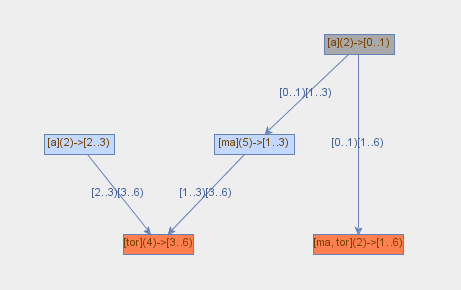
\includegraphics[width=0.7\textwidth]{figures/rosil-amator.png}
    \caption{Graful de tipare pentru cuvântul \textit{amator}}
    \label{fig:rosil-amator}
\end{figure}

La nivelul algoritmului \ref{algo:buildMatchedPatternGraph} este prezentată o metodă prin care se poate construi un graf de tipare pentru un anumit cuvânt pornind de la o mulțime de secvențe frecvente potrivite în cadrul acelui cuvânt. Nodurile grafului rezultat sunt reprezentate de mulțimea inițială de tipare potrivite, iar pentru căile din graf se construiește mulțimea tuturor perechilor de noduri și se filtrează doar cele care se află într-o relație de extensie.

\begin{algorithm}
\SetAlgoLined
\SetKwFunction{ppg}{buildMatchedPatternsGraph}

\ppg($M_w$) \\
\KwData{$M_w$ o colecție de tipare frecvente potrivite în cadrul cuvântului $w$}
\KwResult{$G_w$ un graf de tipare frecvente potrivite în cadrul cuvântului $w$} 

$E_w = \emptyset$ \\
$C_{M_w} = M_w \times M_w$ \\
\For{ $\langle p_1, p_2 \rangle$ in $C_{M_w}$}{
	\If{$p_1 \curvearrowright p_2$} {
		$E_w = E_w \cup $ \{$\langle p_1, p_2 \rangle$\}\\
	}
}
$G_w = \langle M_w, E_w \rangle$ \\
\KwRet $G_w$
\vspace{.1cm}

\caption{Construcția grafului de tipare pentru $w$}
\label{algo:buildMatchedPatternGraph}
\end{algorithm}


\subsection{Interpretarea grafului de tipare frecvente}

Odată construit graful de tipare frecvente, se pune întrebarea dacă pe baza acestuia, se poate dezvolta o metodă de silabisire? 

În graful prezentat în figura \ref{fig:rosil-amator} se pot observa trei dintre cele patru tipuri de tipare (de început, de sfârsit, întermediare), stiind aceasta, se ridică întrebarea dacă caile dintre noduri de început și sfârșit reprezintă posibile despărțiri în silabe, iar dacă, care dintre acestea este despărțirea corectă?

În cazul exemplu prezentat există doua căi între noduri de început si sfârsit, acestea fiind $<a>, <ma, tor>$, respectiv $<a>, <ma>, <tor>$. Din ambele variante se ajunge la despărțirea în silabe $a-ma-tor$, care este si varianta corectă. 

Pornind de la această observație, în cele ce urmează vor fi prezentate o serie de strategii de selecție a căilor dintr-un graf de tipare frecvente care au probabilitate ridicată sa fie despărțiri în silabe corecte. 

Dar până se ajungă la aceste strategii trebuie menționat că în realitate, numărul de tipare frecvente potrivite cu un cuvânt este mult mai mare decât în exemplu demonstrativ din figura \ref{fig:rosil-amator}, iar cum căutarea tuturor căilor între două noduri este o problemă dificilă, a carei soluție depinde de complexitatea grafului analizat, este recomandată o reducere a dimensiunii grafului pentru a reduce complexitatea cautării. 

\subsection{Optimizarea grafului de tipare frecvente}

\begin{figure}[h]
    \centering
    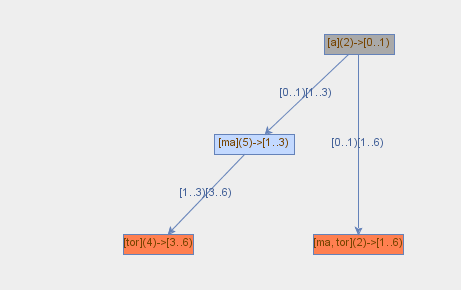
\includegraphics[width=0.6\textwidth]{figures/rosil-amator-prunned.png}
    \caption{Graful de tipare pentru cuvântul \textit{amator}}
    \label{fig:rosil-amator-prunned}
\end{figure}

Pornind de la observația de mai sus și analizând natura grafurile de tipare, se pot identifica două categorii de noduri a căror utilitate este inexistentă în vederea identificării căilor între noduri de început și noduri de sfârsit. Aceste categorii sunt:
\begin{itemize}
\item nodurile la care nu se poate ajunge din niciun nod de start.
\item nodurile din care nu se poate ajunge la niciun nod de sfârșit. 
\end{itemize}

\begin{ex}
În cadrul figurii \ref{fig:rosil-amator-prunned} se poate observa graful de tipare $G_{amator}$ după eliminarea nodurilor izolate.
\end{ex}

Aceste noduri pot fi eliminate fără a altera soluțiile de silabisire identificate. O posibilă soluție pentru eliminarea acestora este descrisă în cadrul algoritmului \ref{algo:prunning}. 

Acesta are două etape: 
\begin{itemize}
\item O primă etapă în cadrul căreia sunt identificate nodurile care nu sunt noduri de sfârșit și nu există nicio muchie care să pornească de la acestea, respectiv nodurile care nu sunt noduri de început și pentru care nu există nicio muchie care să ajungă la ele.
\item Odată identificate aceste noduri, trebuie identificate și muchile care le au ca sursă sau destinație.
\end{itemize}

Eliminând nodurile izolate după aceste două etape, rezultă un graf de dimensiune mai mică. Cele două etape se aplică recursiv până când în cadrul primei etape nu mai este identificat niciun nod izolat. 

\begin{algorithm}[H]
\SetAlgoLined
\SetKwFunction{ppg}{prunePatternGraph}

\ppg($G_{w}$) \\
\KwData{$G_{w}$ un graf de tipare descris prin $\langle V_w, E_w \rangle$}
\KwResult{$G_w'$ un graf fără noduri izolate} 

$isolatedVertices = \emptyset$ \\
\For{ $v$ \textbf{in} $V_w$}{
	\If{$deg^-(v) == 0 \wedge isNotStartNode(v)$} {
		$isolatedVertices = isolatedVertices \cup \{v\}$
	}
	\If{$deg^+(v) == 0 \wedge isNotEndNode(v)$} {
		$isolatedVertices = isolatedVertices \cup \{v\}$
	}
}

\If{$isolatedVertices == \emptyset$} {
	\KwRet $\langle V_w, E_w \rangle$
}


$edgesToBeRemoved = \emptyset$ \\
\For{ $e$ \textbf{in} $E_w$}{
	\If{$e$ \textbf{depends on a vertex from} $isolatedVertices$} {
		$edgesToBeRemoved = edgesToBeRemoved \cup \{e\}$
	}
}

$V_w' = V_w \setminus isolatedVertices$\\
$E_w' = E_w \setminus edgesToBeRemoved$\\

\KwRet \ppg($\langle V_w', E_w'  \rangle$) \\
\vspace{.1cm}

\caption{Eliminarea nodurilor izolate din cadrul unui graf de tipare}
\label{algo:prunning}
\end{algorithm}

\section{Lanțuri închise de tipare secvențiale frecvente}

Pornind de la un graf de tipare, se pot elabora o serie de strategii prin care se stabilește care dintre căile de dintre nodurile de început și sfârșit reprezintă despărțirea corectă în silabe a cuvântului pe baza căruia a fost construit graful de tipare. 

Dar înainte de  a prezenta aceste strategii, este necesară o scurtă analiză a acestor căi.
\subsection{Identificarea căilor care pot reprezenta despărțiri în silabe}

Pentru a putea aplica strategiile menționate mai sus, este necesară identificarea tuturor căilor între nodurile de început și cele de sfârșit. Problema identificării tuturor câilor într-un graf este una dificilă dar în cazul grafurilor de tipare, datorită naturii lor, poate fi abordată (grafurile de tipare sunt grafuri orientate aciclice de dimensiune relativ redusă). 

\begin{defi}
Se notează cu $I_w$ intervalul minim care conține mulțimea tuturor indexilor care pot reprezenta puncte de despărțire pentru cuvântul $w$.
\end{defi}

\begin{defi}
Fie $p_1, p_2, ..., p_n$ o cale într-un graf de tipare $G_w$, cu $p_x$ un tipar potrivit de forma $\langle tipar_x, sup_x, \left[i_x,j_x\right)\rangle$, această cale este un \textbf{lanț de tipare închis} daca 
\begin{equation}
\bigcup_{1 \leq x \leq n} \left[i_x,j_x\right) = I_w
\end{equation}
Cu alte cuvinte, un lanț de tipare închis este o cale într-un graf de tipare, pentru care primul nod este \textit{un nod de început}, iar ultimul nod este \textit{un nod de sfârșit}.
\end{defi}

Cum ar putea fi identificată eficient multimea tuturor lanțurilor de tipare închise? Această întrebare rămâne descrisă. Pentru a valida metoda descrisă în cadrul acestui experiment una dintre variante este ca din fiecare nod start să se realizeze explorări în lătime și reconstrucția lanțurilor de tipare închise pe baza acestor explorări. 

În cadrul algoritmului \ref{algo:findClosedPatternChains} este schițată idea de mai sus.

\begin{algorithm}[H]
\SetAlgoLined
\SetKwFunction{ppg}{findClosedPatternChains}

\ppg($G_w$) \\
\KwData{$M_w$ un graf de tipare frecvente asociat cuvântului $w$}
\KwResult{$L_w$ un set de lanțuri de tipare inchise} 


$L_w = \emptyset$ \\
$SV_{G_w} = findStartVertices(G_w)$ \\
$EV_{G_w} = findEndVertices(G_w)$ \\
$T = SV_{G_w} \times EV_{G_w}$ \\
\For{ $\langle startNode, endNode \rangle$ in $T$}{
	$L_{startNode-endNode} = findPathsBetween(startNode, endNode)$ \\
	$L_w = E_w \cup  \{L_{startNode-endNode}\}$\\
}
\KwRet $L_w$
\vspace{.1cm}

\caption{Identificarea lanturilor de tipare închise din cadrul unui graf de tipare}
\label{algo:findClosedPatternChains}
\end{algorithm}

\subsection{Proprietăți ale lanțurilor de tipare închise}

\begin{defi}
Fie $l$ un lanț de tipare închis dintr-o mulțime $L_w$, notăm cu $s_{l}$ \textbf{silibisirea} cuvântului $w$ folosind $l$. De exemplu având lanțul de tipare închis $\langle <a>, 2, \left[ 0, 1 \right)\rangle, \langle <ma>, 5, \left[ 1, 3 \right)\rangle, \langle <tor>, 4, \left[ 3, 6 \right)\rangle$, silabisirea rezultată este $a-ma-tor$. 
\end{defi}

Ulterior se va utiliza notația $L_w$ pentru mulțimea tuturor lanțurilor de tipare închise din cadrul unui graf $G_w$.

\begin{defi}
Trebuie remarcat că există posibilitatea ca două sau mai multe lanțuri de tipare inchise pot avea aceiași silabisire asociată. Ulterior se va face referire la aceste lanțuri de tipare ca fiind \textbf{echivalente}. Fie $l_1$ și $l_2$ două tipare echivalente, în acest caz se introduce notația $l_1 \equiv l_2$.
\end{defi}

\begin{ex}
Fie $l_1 = \langle <a>, 2, \left[ 0, 1 \right)\rangle, \langle <ma, tor>, 4, \left[ 1, 6 \right)\rangle$, iar $l_2 = \langle <a>, 2, \left[ 0, 1 \right)\rangle, \langle <ma>, 5, \left[ 1, 3 \right)\rangle, \langle <tor>, 4, \left[ 3, 6 \right)\rangle$. Silabisirile asociate sunt $s_{l_1} = a-ma-tor$, respectiv $s_{l_2} = a-ma-tor$, fiind aceleași silabisiri $\Rightarrow l_1 \equiv l_2$.
\end{ex}

\begin{defi}
Considerând $l$ un lanț de tipare închis dintr-o mulțime, $L_w$, notăm cu $\vert l \vert $ \textbf{lungimea} lanțului $l$. Un lanț de lungime 2 este: $\langle <a>, 2, \left[ 0, 1 \right)\rangle, \langle <ma, tor>, 4, \left[ 1, 6 \right)\rangle$.
\end{defi}


\section{Strategii de predictie a despărțirilor în silabe}

\subsection{Strategie bazată pe numărul de căi dintre nodurile extreme}

O primă idee prin care se poate selecta lanțul de tipare închis care să reprezinte silabisirea unui cuvânt, vine de la observația de mai sus cum că din mulțimea completă de lanțuri de tipare inchise, unele sunt echivalente. 

Extinzând observația, se poate pune întrebarea dacă dimensiunea claselor de echivalență poate fi folosită pentru a identifica silabisirea corectă. 

\begin{defi}
Fie $W$ un cuvânt, iar $L_w$ mulțimea tuturor lanțurilor închise identificate din graful de tipare asociat cuvântului $w$. Clasa de echivalență a unui lanț $e$ este 
\begin{equation}
\left[e\right] = \{l \in L_w \vert l \equiv e\}
\end{equation}
Se notează cu $E_{L_w}$\textbf{ mulțimea tuturor claselor de echivalență a lanțurilor de tipare} $L_w$. Se mai notează cu $S_{L_w}$ mulțimea tututor silabisirilor asociate cu $L_w$. 
\end{defi}

În acest context se poate utiliza o relație $f: S_{L_w} \rightarrow E_{L_w}$ pentru a identifica clasa de echivalență asociață cu fiecare silabisire. Utilizând relația $f$, silabisirile posibile ale cuvântului $w$ pot fi ordonate în funcție de cardinalitatea claselor de echivalență. 

Prin acestă strategie se propune ca despărțirea în silabe să fie dată de cea mai numeroasă clasa de echivalentă.

\begin{ex}
În cadrul figurii \ref{fig:rosil-counting} este ilustrată aplicarea acestei strategii. 
\end{ex}

\begin{figure}[h!]
    \centering
    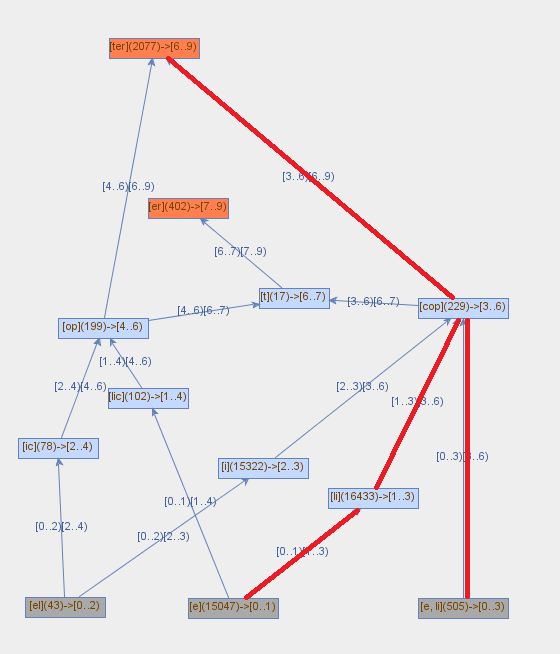
\includegraphics[width=0.6\textwidth]{figures/rosil-counting.png}
    \caption{Aplicarea strategiei numărului de lanțuri închise pentru $G_{elicopter}$}
    \label{fig:rosil-counting}
\end{figure}

\subsection{Strategie bazată pe nivelul de suprapunere}

O altă strategie pornește de la presupunerea că un nivel ridicat de suprapunere la între tiparele unui lanț închis duce la o mai bună predicție a silabisirii unui cuvânt.

\begin{defi}
Având două tipare potrivite în cadrul unui cuvânt la pentru intervalul de îndexi $[i_{p_1}, j_{p_1})$, respectiv $[i_{p_2}, j_{p_2})$ de definește nivelul de potrivire al acestor două tipare ca fiind:
\begin{equation}
\omega(p_1, p_2) = \left\{
\begin{matrix}
0, 					& j_{p_1} \leq i_{p_2}\\ 
max(i_{p_2},j_{p_1)} - min(j_{p_2},i_{p_1}),	& j_{p_1} > i_{p_2} \\
\end{matrix}
\right.
\end{equation}
\end{defi}

\begin{ex}
Pentru tiparul $p_1$ potrivit la întervalul $\left[0, 6\right)$ și tiparul $p_2$ potrivit la întervalul $\left[4, 8\right)$ avem $ \omega(p_1,p_2)=2$
\end{ex}

\begin{defi}
Fie $p_1, p_2, ..., p_n$ un lant de tipare închis $l$. Nivelul de suprapunere pentru întreg lanțul este:
\begin{equation}
\Omega(l) = \sum_{i=1}^{n-1}{ \omega(p_i, p_{i+1})}
\end{equation}
\end{defi}

\begin{figure}[h!]
    \centering
    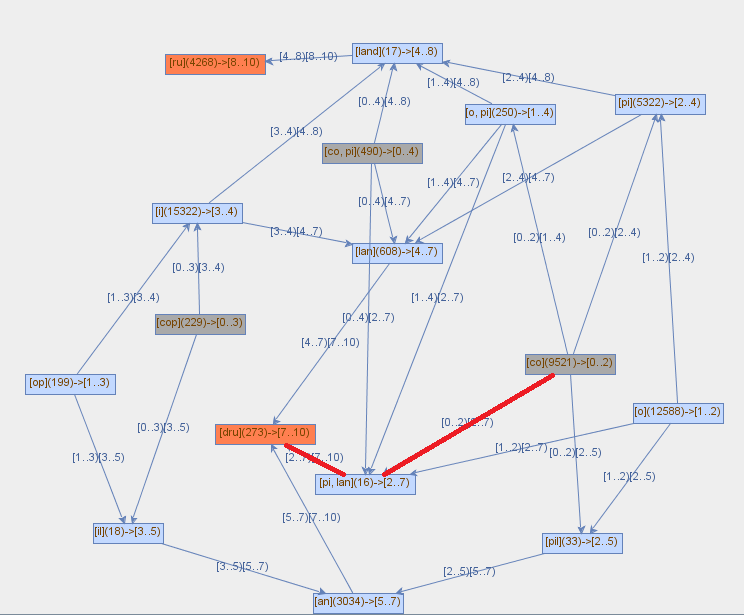
\includegraphics[width=0.7\textwidth]{figures/rosil-overlapping.png}
    \caption{Aplicarea strategiei bazate pe nivelul de suprapunere pentru $G_{copilandru}$}
    \label{fig:rosil-overlapping}
\end{figure}

Pornind de la definiția nivelului de suprapunere de la nivelul unui lanț de tipare închis, se poate realiza o ordonare in funcție de acest nivel a lanțurilor închise din cadrul unui graf de tipare al unui cuvânt, iar ulterior să se propună ca silabisire a acelui cuvânt, silabisirea asociată cu lanțul închis cu nivel maxim de suprapunere. Această strategie este ilustrată în cadrul \ref{fig:rosil-overlapping}.




\subsection{Strategie bazată pe distanța dintre nodurile extreme}

A treia strategie propusă încearcă să exploreze presupunerea că, cu cât sunt mai lungi tiparele dintr-un lant închis, cu atât creste probabilitatea ca acest lanț să aibă asociată o silabisire corectă.

Dar cum s-ar putea identifica aceste lanțuri? Un posibil răspuns la această întrebare vine de la observația că lungimea medie a tiparelor dintr-un lanț inchis este invers proporțioanală cu lungimea lanțului. 

Atfel, acestă stategie selecția acelor lanțuri de lungime minimă. Deasemenea, în cazul în care există mai multe lanțuri de lungime minimă, se va alege acela care prezintă mai mai mare grad de suprapunere. 

\begin{ex}
În cadrul figurii \ref{fig:rosil-shortest} este ilustrată aplicarea acestei strategii. 
\end{ex}

\begin{figure}[h]
    \centering
    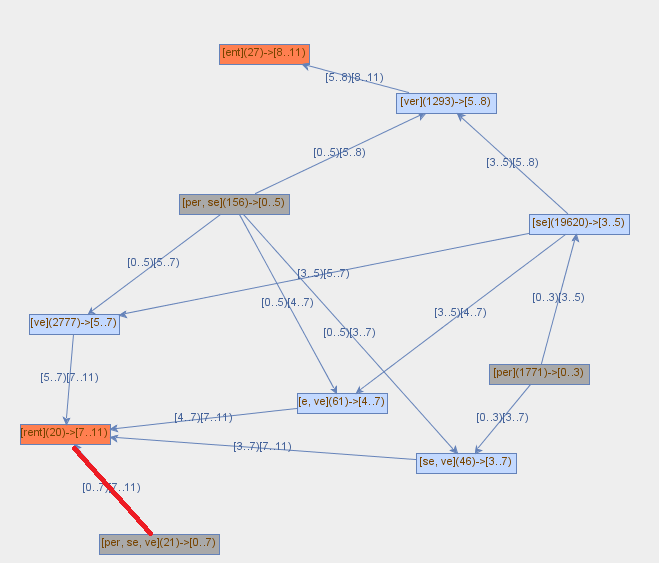
\includegraphics[width=0.8\textwidth]{figures/rosil-shortest.png}
    \caption{Aplicarea strategiei drumului minim pentru $G_{perseverent}$}
    \label{fig:rosil-shortest}
\end{figure}

\section{Metrici de evaluare}

Odată definite strategiile de mai sus, acestea trebuie validate, iar pentru a le valida, se vor defini doua metrici.

\subsection{Evaluare la nivel de cuvânt}


Cea mai simplă variantă este de a considera de a trata despărțirea în silabe ca fiind atomică.

\begin{defi} Fie $w$ un cuvânt, iar $s_p$ o silabisire posibilă a acestui, și $s_e$ silabisirea corectă. Atunci, se definește metrica de evaluare a silabisirii propuse ca fiind:

\begin{equation}
m_w(s_p,s_e) = \left\{
\begin{matrix}
0, 	& $ dacă $ s_p=s_e\\ 
1,	& $ dacă $ s_p\neq s_e \\
\end{matrix}
\right. 
\end{equation}
\end{defi}

\subsection{Evaluare la nivel de punct de despărțire}

În anumite cazuri există mai multe despărțiri în silabe corecte (în funcție de context), este necesară si definirea unei metrici cu o granularitate mai mică.

\begin{defi}
Fie $s$ o despărțire în silabe a unui cuvânt. Mulțimea punctelor de despărțire echivalente despărțirii $s$ este colecția de indexilor acelor litere din cuvânt, care au înaintea lor un punct de despărțire. De exemplu pentru despărțirea $a-ma-tor$, mulțimea punctelor de despărțire este $\{1,3\}$.
\end{defi}


\begin{defi}
Considerând mulțimea indexilor de despărțire $I_{s_p}$ pentru o silabisire $s_p$ a unui cuvânt, iar $I_{s_e}$ mulțimea indexilor despărțirii corecte a aceluiași cuvânt, se definește metrica $m_d$:

\begin{equation}
m_d(s_p,s_e) = 1- \frac{\vert I_{s_e} \setminus I_{s_p} \vert}{2 \cdot \vert I_{s_e} \vert} - \frac{\vert I_{s_p} \setminus I_{s_e} \vert}{2 \cdot \vert I_{s_p} \vert}
\end{equation}
\end{defi}

Interpretarea metricii de mai sus depinde de două componente: numărul de puncte de despărțire prezise corect și numărul de puncte de despărțire prezise gresit.

\begin{ex}
Pentru o mai bună întelegere, fie următoarele exemple:

\begin{equation}
m_d(\{1,3,5\}, \{2,4,6\}) = 1- \frac{3}{2 \cdot 3} - \frac{3}{2 \cdot 3} = 0 
\end{equation}

\begin{equation}
m_d(\{1,3,5\}, \{2,3,6\}) = 1- \frac{2}{2 \cdot 3} - \frac{2}{2 \cdot 3} \simeq 0.33 
\end{equation}

\begin{equation}
m_d(\{1,3,5\}, \{2,3,5\}) = 1- \frac{1}{2 \cdot 3} - \frac{1}{2 \cdot 3} \simeq 0.66 
\end{equation}


\begin{equation}
m_d(\{1,3,5\}, \{1,3,5\}) = 1 - \frac{0}{2 \cdot 3} - \frac{0}{2 \cdot 3} = 1 
\end{equation}


\end{ex} 

\section{Algoritm de silabisire folosind tipare secvențiale frecvente}
În \ref{algo:rosil} este ilustrat algoritmul complet prin care se poate identifica silabisirea unui cuvânt pornind de la o colecție de tipare secvențiale frecvente și o strategie prin care se alege o silabisire din cadrul mulțimii silabisirilor posibile identificate pe baza tiparelor frecvente.

Pentru implementarea acestuia se pot utiliza algoritmii mai sus descriși:

\begin{itemize}
\item Identificarea tiparelor potrivite: algoritmul~\ref{algo:findMatchedPatterns}
\item Construirea grafului de tipare: algoritmul~\ref{algo:buildMatchedPatternGraph}
\item Optimizarea grafului de tipare: algoritmul~\ref{algo:prunning}
\item Identificarea lanțurilor de tipare închise: algoritmul~ \ref{algo:findClosedPatternChains}
\end{itemize}


\begin{algorithm}
\SetAlgoLined
\SetKwFunction{ppg}{splitWord}

\ppg($P, w$) \\
\KwData{$P$ o colecție de tipare secvențiale frecvente, $w$ cuvântul care se dorește a fi despărțit în silabe, $selectionStrategy$ o strategie de selecție a unei silabisiri din cadrul unei colecții de lanțuri închise de tipare}
\KwResult{$s_w$ o silabisire a cuvântului $w$} 

$M_w = findMatchingPatterns(P,w)$ \\
$G_w = buildMatchedPatternsGraph(M_w)$ \\
$Gp_w = prune(G_w)$ \\
$L_w = findClosedPatternChains(Gp_w)$ \\
\KwRet $pickSolution(L_w, selectionStrategy)$
\vspace{1cm}

\caption{Predicția despărțirii în silabe ale unui cuvânt $w$}
\label{algo:rosil}
\end{algorithm}

Având o soluție pentru identificarea unei silabificări ale unui cuvând pornind de la un set indexat de tipare frecvente, este necesară obținerea acestora în prima fază. Acesta poate fi obținută cu ajutorul algoritmului ~\ref{algo:fse}. Indexarea acestora nu este descrisă aici, reprezentând doar utilizarea unei structuri cum ar fi o tabelă de dispersie pentru a stoca tipare identificate. 

\chapter{Detalii de proiectare si implementare}

În vederea validării ideilor mai sus prezentate, a fost realizată o implementare în limbajul Java care este descrisă în cele ce urmează.

\section{Tehnologii utilizate}

Soluția a fost implementată folosind următoarele tehnologii:

\begin{itemize}
	\item \textit{JDK 8} ~\footnote{https://jdk8.java.net/}
	\item \textit{Gradle} ~\footnote{https://gradle.org/} (pentru compilare si impachetare)
	\item \textit{Git} ~\footnote{https://git-scm.com/} (pentru versionare)
\end{itemize}

La nivel de librarii Java au fost folosite următoarele librarii:

\begin{itemize}
    \item \textit{com.google.guava:guava:18.0} (pentru colecții)
	\item \textit{org.apache.commons:commons-lang3:3.4} (pentru manipulare de siruri de caractere)
    \item \textit{com.google.code.gson:gson:1.7.2} (pentru serializare JSON)
    \item \textit{jgraph:jgraph:5.13.0} (pentru abstractizare și manipulare de grefuri)
	\item \textit{org.jgrapht:jgrapht-dist:0.9.1} (pentru visualizare de 
grafuri)
	\item \textit{jp.ac.titech.cs.se:sparesort:0.2.0} (pentru identicarea de tipare secvențiale frecvente)
	\item \textit{org.apache.logging.log4j:log4j-core:2.3} (pentru logare)
    \item \textit{junit:junit:4.12} (pentru unit-teste)
\end{itemize}

Codul sursă al projectului poate fi consultat la urmatoarea adresa: \begin{center}
\textbf{\href{https://github.com/adrianulbona/rosil}{https://github.com/adrianulbona/rosil}}
\end{center}

\section{Organizarea aplicației}

Aplicația implementată în cadrul acestui proiect este organizată în patru pachete, ilustrate în figura \ref{fig:rosil-packages}.

\begin{figure}[h!]
    \centering
    
\includegraphics[width=0.9\textwidth]{figures/rosil-packages.png}
    \caption{Pachetele Java ale prototipului implementat}
    \label{fig:rosil-packages}
\end{figure}

Pachetul \textit{input} este utilizat pentru a citi setul de cuvinte silabisite si pentru al pregatii pentru procesari ulterioare. Pachetul \textit{pattern} are ca principala responsabilitate identificarea tiparelor secvențiale frecvente din cadrul cuvintelor deja sibabisite si incărcate cu ajutorul pachetului \textit{input}. Componenta de predicție este localizată în cadrul pachetului \textit{predict}, iar în cadrul pachetului \textit{eval} au fost implementate o serie de metrici necesare validarii diverselor strategii de predictie.

\begin{figure}[h!]
    \centering
    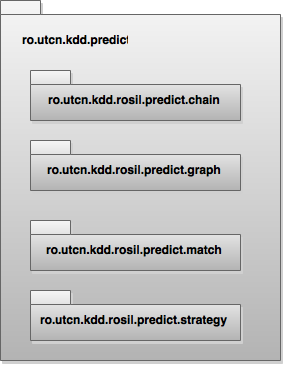
\includegraphics[width=0.35\textwidth]{figures/rosil-predict-packages.png}
    \caption{Organizarea pachetului \textit{predict}}
    \label{fig:rosil-predict-packages}
\end{figure}

Pachetul \textit{predict} este deasemenea compus din mai multe sub-pachete care sunt ilustrate în diagrama ~\ref{fig:rosil-predict-packages}. 

Sub-pachetul \textit{match} are ca responsabilitate identificarea tiparelor (dintr-o colectie de tipare) care potrivesc un anumit cuvânt, sub-pachetul \textit{graph} modeleaza grafuri de tipare potrivite, în cadrul sub-pachetului \textit{chain} conține abstractizari pentru lanțuri de tipare, iar sub-pachetul \textit{strategy} conține implementari pentru strategiile de selecție ale unei silabificari dintr-o colecție de lanțuri de tipare. 

\section{Impachetarea aplicației - modularizare}

Prototipul implementat a fost conceput într-o perspectivă modulară. Prin această se dorește o separare a părții în efective de predicție de silabisiri de partea de interfață cu utilizatorul. 

Astfel aplicația poate fi împachetată ca o simplă aplicație desktop după cum este ilustrat în figura \ref{fig:rosil-desktop}.

\begin{figure}[h!]
    \centering
    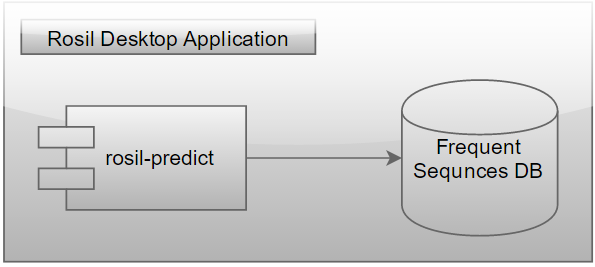
\includegraphics[width=0.55\textwidth]{figures/rosil-desktop.png}
    \caption{Modulul de predicție a silabisirii ca aplicație desktop}
    \label{fig:rosil-desktop}
\end{figure}

Dar aceiași componentă poate fi utilizată pentru a construi un serviciu WEB care este accesibil prin internet. În cadrul figurii \ref{fig:rosil-service}

\begin{figure}[h!]
    \centering
    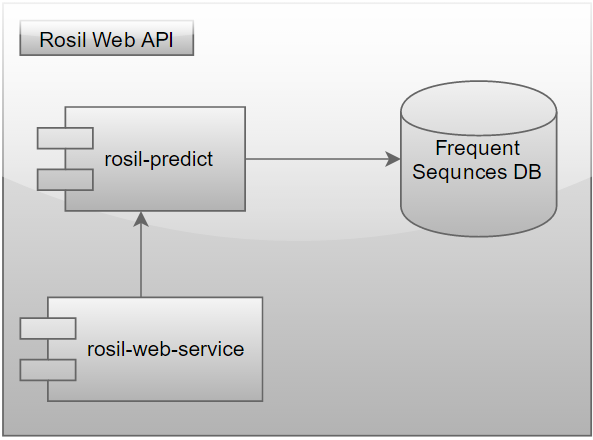
\includegraphics[width=0.50\textwidth]{figures/rosil-service.png}
    \caption{Modulul de predicție a silabisirii ca serviciu web}
    \label{fig:rosil-service}
\end{figure}

\section{Ghid de utilizare}

Pentru a executa aplicația, în primă faza este necesară descărcarea codului acesteia. Pentru această este necesar ca utilitarul Git sa fie instalat, odată acesta instalat se poate executa următoarea comanda:

\begin{center}
\textbf{git clone https://github.com/adrianulbona/rosil.git}
\end{center} 

Odată descărcată aplicația, din directorul acesteia poate fi executată următoarea comanda pentru a obtine despărți în silabe un anumit cuvânt:

\begin{center}
\textbf{gradle run -Dword=\textit{castravete}}
\end{center} 

Rezultatul acestei comenzi are două componente. În primă fază este afișat graful de tipare frecvente pentru cuvântul specificat, similar cu cel din figura 

\begin{figure}[h!]
    \centering
    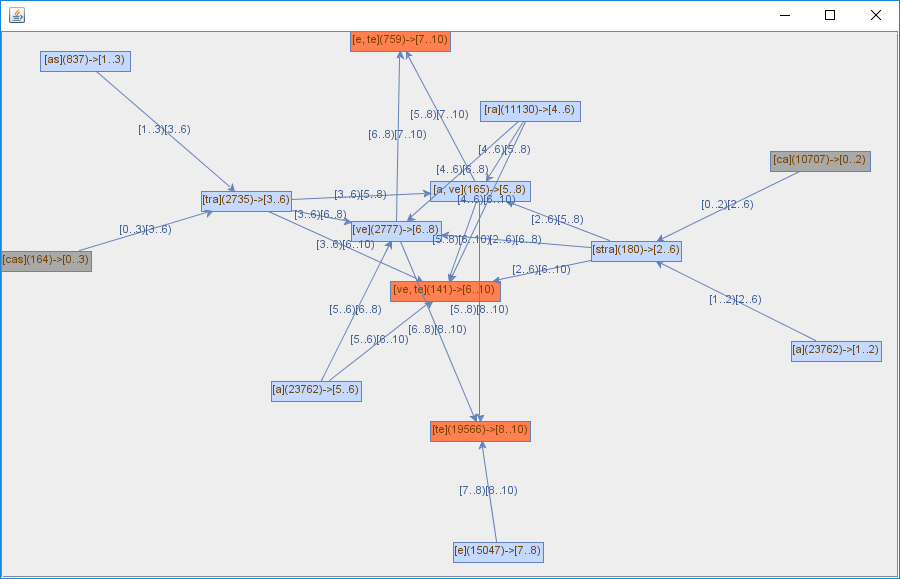
\includegraphics[width=1.0\textwidth]{figures/rosil-castravete.png}
    \caption{Exemplu de vizualizare a unui graf de tipare frecvente în timpul execuției}
    \label{fig:rosil-service}
\end{figure}


\textbf{18:59:17.692 [main] - Reading patterns...}

\textbf{18:59:20.924 [main] - count: ca-stra-ve-te}

\textbf{18:59:20.963 [main] - length: ca-stra-ve-te}

\textbf{18:59:20.969 [main] - overlapping: ca-stra-ve-te}

Se poate observa că pentru fiecare dintre strategiile de selecție a silabisiri este afișat rezultatul. 

Ar mai trebui precizat că, de fiecare dată când se pornește aplicația, colecția de secvențe frecvente este încărcată în memorie, ceea ce durează semnificativ relativ la cât durează predicția efectivă. Acest lucru poate fi optimizat dacă aplicația nu ar fi pornită la fiecare predicție.

\section{Silabisirea ca serviciu web}

După cum a fost prezentat la nivelul diagramei din figura~\ref{fig:rosil-service} modulul de predicție al prototipului implementat, poate fi încapsulat în cadrul unui/unor servicii web.

Această abordare prezintă o serie de avantaje, printre care merită menționate următoarele:

\begin{itemize}
\item accesibilitate: un serviciu web poate fi accesibil de oriunde, având o conexiune la internet
\item scalabilitate: un serviciu web poate fi scalat în funcție de volumul de cereri. 
\end{itemize}

Prototipul implementat explorează și posibilitatea construirii unui astfel de serviciu web, iar odată cu execuția comenzii:

\begin{center}
\textbf{gradlew rosil-api:run}
\end{center}

Serviciul web este pornit cu ajutorul comenzii anterioare poate fi accesat cu ajutorul unui browser sau cu următoarea comanda:

\begin{center}
\textbf{curl http://localhost:4567/rosil/castravete}
\end{center}

Iar rezultatul prezintă variante de silabisire alte cuvântului /textit{castravate} în formatul JSON:


\textbf{\{}

\hspace{1cm}\textbf{"shortest": "cas-tra-ve-te",}

\hspace{1cm}\textbf{"overlapping": "cas-tra-ve-te",}

\hspace{1cm}\textbf{"counting": "cas-tra-ve-te",}
 
\textbf{\}}

\section{Implentarea unui serviciu web de silabisire}

La nivel de implementare pentru a fost utilizată libraria \textbf{spark~\footnote{http://sparkjava.com/}}, care oferă posibilitatea construiti de servicii web cu usurintă după cum este ilustrat în cadrul secvenței de cod Java~\ref{fig:rosil-api}.

\begin{figure}[h!]
    \centering
    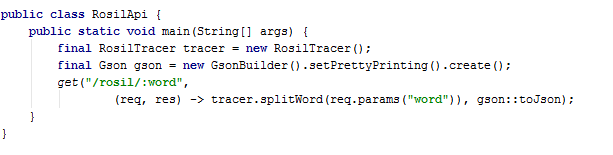
\includegraphics[width=1.06\textwidth]{figures/rosil-api-code.png}
    \caption{Secvență de cod Java 8 utilizată pentru construirea serviciului web de silabisire}
    \label{fig:rosil-api}
\end{figure}

Întreg serviciu web se foloșeste de clasa \textbf{RosilTracer} care oferă silabisiri pentru un cuvânt, iar de fiecare dată când o cerere de forma \textbf{rosil/\textit{cuvânt}}, rezultatul opținut este serializat în format JSON și este trimis inapoi apelantului.

Similar cu acest serviciu, aplicația web poate fi extinsă cu o serie de servicii care să expună mai multă informație decât predicțiile finale. Spre exemplu, graful de tipare ar putea fi acesat de la un serviciu similar cu cel prezentat anterior. Un graf de tipare expus prezintă avanțajul că oricine l-ar putea folosi pentru a-și construi proprile strategii de predicție a silabisirii. 
% \chapter{Tests and Results}
\chapter{Rezultate teoretice și experimentale}
\label{cap:rezultate}

Împreună cu partea de prezentare a proiectului, trebuie să reprezinte aproximativ 70\% din lucrare. 

Aici sunt prezentate metodele de validare a soluțiilor/sistemului descris în capitolele anterioare, scenariile de testare a corectitudinii funcționale, a utilizabilității, performanței etc.   

Rezultatele testelor experimentale necesită, în general interpretări (dacă rezultatele obținute corespund așteptărilor, intuițiilor cititorului, de ce apar variații/excepții etc.) și comparații cu rezultatele altor metode similare. 

Sistemele de testare și testele propriu-zise trebuie descrise detaliat astfel încât să poată fi reproduse și de alții care poate vor să-și compare soluțiile lor cu a voastră (eventual, codul testelor poate fi pus în anexe). Dacă se poate alegeți pentru evaluarea sistemului vostru benchmark-uri (pachete de testare) dedicate, astfel încât comparația cu alte sisteme să poată fi făcută mai ușor. În plus, astfel de teste sunt mult mai complete și mai realiste decât cele dezvoltate de voi. Oricum, încercați ca testele efectuate să nu fie triviale, ci să acopere scenarii cât mai reale, mai complexe și mai relevante ale funcționării sistemului vostru. 

% \section{Functional Tests}
\section{Teste de funcționalitate}



% \section{Performance Tests}
\section{Teste de performanță}
\chapter{Concluzii si direcții posibile de urmat}
\label{cap:concluzii}

În cadrul acestei lucrări a fost explorată problema silabisirii și a fost propusă o metodă prin care această problemă poate fi rezolvată. Au fost descrise conceptele teoretice utilizate la construcția soluției, a fost realizată o implementare a metodei și au fost evaluate rezultatele acesteia. 

Trebuie menționat că soluția propusă, deși nu oferă cea mai ridicată precizie, comparativ cu alte abordări, vine cu o serie de avantaje: genericitate, nedepinzând de regulile specifice ale unei limbi, performanță la nivelul timpului de execuție și extensibilitate.

Pentru viitor munca existentă ar putea fi continuată în câteva direcții:

\begin{itemize}
\item Definirea unor \textit{contexte} de silabisire. Silabisirea nu se bazează pe un set de reguli clare, dar asociind anumite reguli cu un anumit context și aborband acele contexte diferit, s-ar putea îmbunătăți precizia soluției.

\item Validarea metodei în cadrul unor limbi non-indoeuropene. 

\item Dezvoltarea unei aplicații web prin care grafurile de tipare sa poată fi analizate de către specialiștii din lingvistică. 



\end{itemize}











\bibliographystyle{IEEEtran}
\bibliography{thesis}

\appendix

\chapter{Pseudo-cod sau cod (dacă există)}

\begin{lstlisting}
 /** Maps are easy to use in Scala. */
object Maps {
  val colors = Map("red" -> 0xFF0000,
                   "turquoise" -> 0x00FFFF,
                   "black" -> 0x000000,
                   "orange" -> 0xFF8040,
                   "brown" -> 0x804000)
  def main(args: Array[String]) {
    for (name <- args) println(
      colors.get(name) match {
        case Some(code) =>
          name + " has code: " + code
        case None =>
          "Unknown color: " + name
      }
    )
  }
}
\end{lstlisting}



\end{document}
